\documentclass[xcolor={dvipsnames,table},aspectratio=169]{beamer}
\usepackage[utf8]{inputenc}
\usepackage[T1]{fontenc}
\usepackage[brazil]{babel}
\usepackage{graphics,amssymb,amsfonts,amsmath}
\usepackage{enumerate,hyperref}
\usepackage{palatino}
\usepackage{ragged2e}
\usepackage{minted}
\usepackage{booktabs}
\usepackage{verbatim}
%\usepackage{listings}
\usepackage[export]{adjustbox}
\usepackage{tikz}                   
\usepackage{xcolor}
\usepackage{textcomp} % para usar \textdegree
\usetikzlibrary{shadows}
\usetheme{AnnArbor}
\usecolortheme{orchid}
\usefonttheme[onlymath]{serif}

\newminted{java}{bgcolor=cyan!10}

\newcolumntype{C}[1]{>{\centering\let\newline\\\arraybackslash\hspace{0pt}}m{#1}}

\AtBeginSection[]{
  \begin{frame}
  \vfill
  \centering
  \begin{beamercolorbox}[sep=8pt,center,shadow=true,rounded=true]{title}
    \usebeamerfont{title}\insertsectionhead\par%
  \end{beamercolorbox}
  \vfill
  \end{frame}
}

\title[\sc{Decisões}]{Decisões}
\author[Roland Teodorowitsch]{Roland Teodorowitsch}
\institute[FPROG - EP - PUCRS]{Fundamentos de Programação - Escola Politécnica - PUCRS}
\date{6 de setembro de 2022}

\begin{document}
\justifying

%-------------------------------------------------------
\begin{frame}
	\titlepage
\end{frame}

%=======================================================
\section{Introdução}

%-------------------------------------------------------
\begin{frame}\frametitle{Objetivos}
\begin{itemize}
	\item Implementar decisões (simples e complexas) usando o comando \texttt{if}
	\item Comparar números inteiros e de ponto-flutuante, e cadeias de caracteres
	\item Escrever comandos usando o tipo de dado \texttt{boolean}
	\item Desenvolver estratégias para testar seus programas
	\item Validar a entrada do usuário
\end{itemize}
\end{frame}

%-------------------------------------------------------
\begin{frame}\frametitle{Conteúdos}
\begin{itemize}
	\item Motivação
	\item O Comando \texttt{if}
	\item Comparando Números
	\item Comparando \emph{Strings}
	\item Múltiplas Alternativas
	\item Decisões Aninhadas
	\item Solução de Problemas: Casos de Teste
	\item Variáveis e operadores Booleanos
	\item Aplicação: Validação da Entrada
\end{itemize}
\end{frame}

%=======================================================
\section{Motivação}

%-------------------------------------------------------
\begin{frame}\frametitle{Motivação}
\begin{itemize}
	\item Considere um programa para calcular as raízes reais de uma equação do segundo grau\\$ax^2 + bx + c = 0$ (com $a\neq 0$)
	\item A solução pode ser obtida com a fórmula de Bhaskara
\[x=\frac{-b\pm\sqrt{\Delta}}{2a}\]
onde $\Delta = b^2-4ac$
\end{itemize}
\end{frame}
	
%-------------------------------------------------------
\begin{frame}[fragile]\frametitle{Implementação 1}
\pause
\tiny{
\inputminted[bgcolor=cyan!10]{java}{src/Bhaskara.java}
}
\end{frame}
	
%-------------------------------------------------------
\begin{frame}\frametitle{Mas...}
\begin{itemize}
	\item O valor de $\Delta$ determina se:
	\begin{itemize}
		\item há duas raízes reais ($\Delta > 0$)
		\item há uma raiz real ($\Delta = 0$) ou
		\item NÃO há raízes reais ($\Delta < 0$)
	\end{itemize}
	\item Então o programa funcionaria melhor se o valor de $\Delta$ fosse testado!
\end{itemize}
\end{frame}
	
%-------------------------------------------------------
\begin{frame}[fragile]\frametitle{Implementação 2}
\pause
\tiny{
\inputminted[bgcolor=cyan!10]{java}{src/Bhaskara2.java}
}
\end{frame}
	
%=======================================================
\section{O Comando if}

%-------------------------------------------------------
\begin{frame}\frametitle{Decisões}
\begin{itemize}
	\item Um programa de computador frequentemente necessita tomar decisões baseadas em alguma entrada ou em dados sendo processados
	\item Exemplos:
	\begin{itemize}
		\item Calcular as raízes de uma equação do segundo grau ($a.x^2 + b.x + c = 0$) com delta podendo ser maior do que zero, igual a zero ou menor do que zero
		\item Mostrar a mensagem ``Aprovado'', se o aluno tem nota de g1 maior ou igual a 7,0; ou a mensagem ``G2 ou Reprovado'', em caso contrário
		\item Nos EUA, por superstição, frequentemente os prédios pulam o 13\textdegree andar, e os elevadores devem lidar com isto (o 14\textdegree andar é, na verdade, o 13\textdegree andar: se $andar > 13$, então $andar = andar - 1$)
		\item Calcular o valor de uma multa e o número de pontos de um motorista que passa a uma certa velocidade acima do limite de uma via
		\item etc.
	\end{itemize}
	\item Para situações como estas, que exigem decisões, usa-se o comando \texttt{if}, que muitas vezes vem acompanhado de um \texttt{else}
\end{itemize}
\end{frame}

%-------------------------------------------------------
\begin{frame}\frametitle{O Comando \texttt{if}}
\begin{itemize}
	\item O principal comando de decisão em Java é o comando \texttt{if} (losango nos fluxogramas)
	\item O comando \texttt{if} deve especificar uma condição (expressão que gera um \texttt{boolean}) entre parênteses e um comando ou bloco para ser executado se a condição for verdadeira (\texttt{true})\\
\texttt{if ( delta < 0.0 )\\~~~System.out.println("SEM raizes reais");}\\
	\item \texttt{else} pode ser usado para especificar o que fazer se a condição for falsa (\texttt{false})\\
\texttt{if ( g1 >= 7.0 )\\~~~System.out.println("Aprovado");\\else\\~~~System.out.println("G2 ou Reprovado");}\\
\end{itemize}
\end{frame}


%-------------------------------------------------------
\begin{frame}\frametitle{Fluxogramas}
\begin{itemize}
	\item Já vimos alguns exemplos de fluxogramas
	\item Um fluxograma mostra a estrutura de tarefas e decisões que tem que ser executadas para resolver um problema
	\item Os elementos básicos de um fluxograma são:
\begin{figure}[h]
	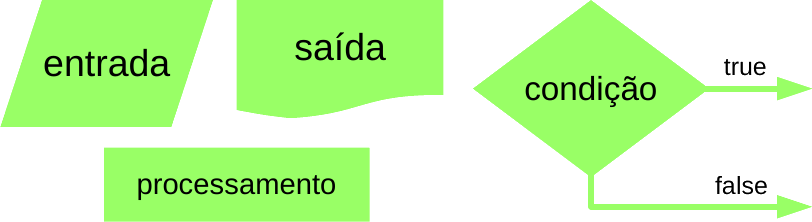
\includegraphics[height=0.25\paperheight,center]{pucrs-ep-fprog-unidade_03-decisoes-laminas-elementos_de_fluxogramas.png}
\end{figure}
	\item Os elementos de um fluxograma são conectados com setas
	\item Nunca aponte uma seta para dentro de outro ramo (isto cria ``código spaghetti'', que dificulta entendimento e manutenção)
\end{itemize}
\end{frame}

%-------------------------------------------------------
\begin{frame}[fragile]\frametitle{Fluxograma do comando \texttt{if}}
\begin{itemize}
	\item Um comando \texttt{if} pode não necessitar fazer nada se a condição for falsa
\begin{columns}
\begin{column}{0.4\textwidth}
	\begin{center}
	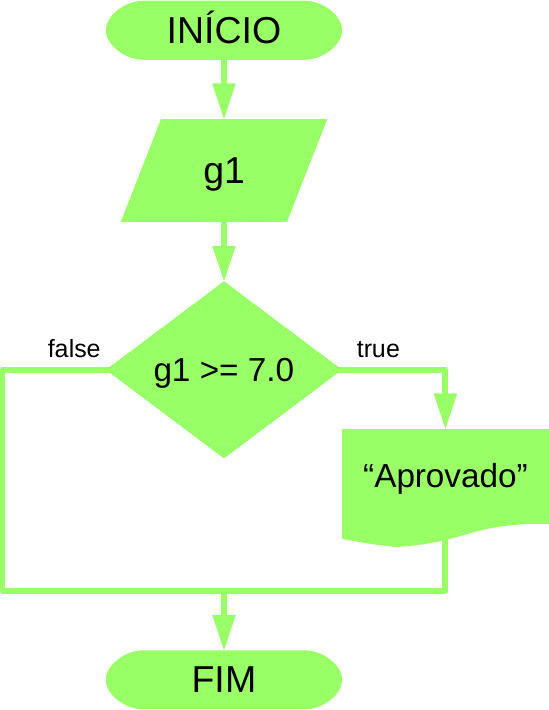
\includegraphics[height=0.6\paperheight]{pucrs-ep-fprog-unidade_03-decisoes-laminas-fluxograma_if.png}
	\end{center}
\end{column}
\begin{column}{0.6\textwidth}
	\footnotesize{\inputminted[bgcolor=cyan!10]{java}{src/Aprovado.java}}
\end{column}
\end{columns}
\end{itemize}
\end{frame}

%-------------------------------------------------------
\begin{frame}[fragile]\frametitle{Fluxograma do comando \texttt{if} com \texttt{else}}
\begin{itemize}
	\item Um comando \texttt{if} pode especificar o que fazer quando a condição for verdadeira e o que fazer quando ela for falsa (\texttt{else})
\begin{columns}
\begin{column}{0.4\textwidth}
	\begin{center}
	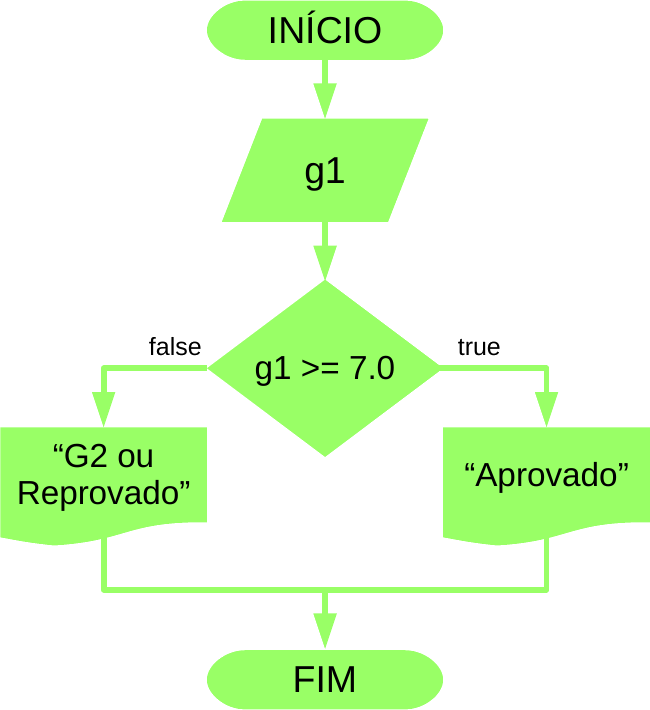
\includegraphics[height=0.6\paperheight]{pucrs-ep-fprog-unidade_03-decisoes-laminas-fluxograma_if_else.png}
	\end{center}
\end{column}
\begin{column}{0.6\textwidth}
	\tiny{\inputminted[bgcolor=cyan!10]{java}{src/AprovadoOuNao.java}}
\end{column}
\end{columns}
\end{itemize}
\end{frame}

%-------------------------------------------------------
\begin{frame}[fragile]\frametitle{Fluxograma com mais de 2 ``ramos''}
\begin{itemize}
	\item Quando há mais de duas opções pode-se usar um \texttt{if}/\texttt{else} dentro de um \texttt{if} e/ou \texttt{else}
\begin{columns}
\begin{column}{0.4\textwidth}
	\begin{center}
	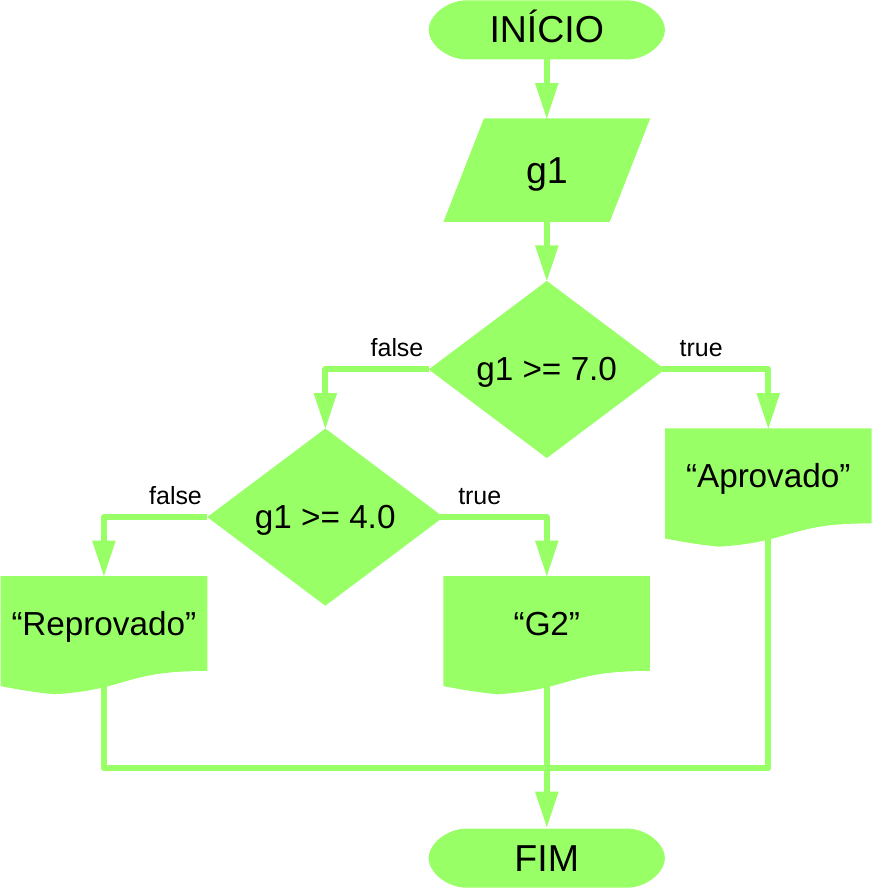
\includegraphics[height=0.6\paperheight]{pucrs-ep-fprog-unidade_03-decisoes-laminas-fluxograma_if_else_aninhado.png}
	\end{center}
\end{column}
\begin{column}{0.6\textwidth}
	\tiny{\inputminted[bgcolor=cyan!10]{java}{src/AprovadoG2OuReprovado.java}}
\end{column}
\end{columns}
\end{itemize}
\end{frame}

%-------------------------------------------------------
\begin{frame}\frametitle{Fluxograma com mais ramos}
\begin{center}
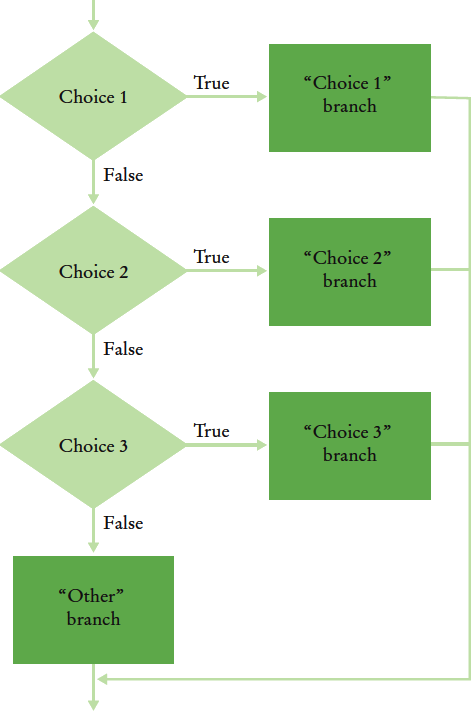
\includegraphics[height=0.6\paperheight]{pucrs-ep-fprog-unidade_03-decisoes-laminas-if_com_varios_ramos.png}
\end{center}
\end{frame}

%-------------------------------------------------------
\begin{frame}[fragile]\frametitle{\texttt{ElevatorSimulation.java} {\tiny (HORSTMANN, 2013, p. 84-85)}}
{\tiny
\begin{javacode}
import java.util.Scanner;

/**
   This program simulates an elevator panel that skips the 13th floor.
*/
public class ElevatorSimulation {
   public static void main(String[] args) {
      Scanner in = new Scanner(System.in);
      System.out.print("Floor: ");
      int floor = in.nextInt();

      // Adjust floor if necessary
      int actualFloor;
      if (floor > 13) {
         actualFloor = floor - 1;
      }
      else {
         actualFloor = floor;
      }
      System.out.println("The elevator will travel to the actual floor " + actualFloor);
   }
}
\end{javacode}
}
\end{frame}

%-------------------------------------------------------
\begin{frame}[fragile]\frametitle{Dicas sobre o Uso de Chaves}
\begin{itemize}
	\item É uma boa prática alinhar todos os pares de chaves verticalmente
	\begin{itemize}
		\item Alinhados
\begin{javacode}
if (floor > 13)
{
   floor--;
}
\end{javacode}
		\item Não alinhados (economizando linhas)
\begin{javacode}
if (floor > 13) {
   floor--;
}
\end{javacode}
	\end{itemize}
\end{itemize}
\end{frame}

%-------------------------------------------------------
\begin{frame}[fragile]\frametitle{Dicas sobre o Uso de Chaves}
\begin{itemize}
	\item Mesmo que para seleção de um único comando não seja necessário, sempre use chaves
	\begin{itemize}
		\item Em vez de
\begin{javacode}
if (floor > 13)
   floor--;
\end{javacode}
		\item Prefira usar
\begin{javacode}
if (floor > 13)
{
   floor--;
}
\end{javacode}
	\end{itemize}
\end{itemize}
\end{frame}

%-------------------------------------------------------
\begin{frame}\frametitle{Dicas sobre Blocos Indentados}
\begin{itemize}
	\item O código Java é estruturado em blocos
	\item Use a tecla \texttt{Tab} para criar uma indentação consistente com número adequado de espaços
	\item Uma indentação consistente torna o entendimento do código muito mais fácil para humanos
\begin{figure}[h]
	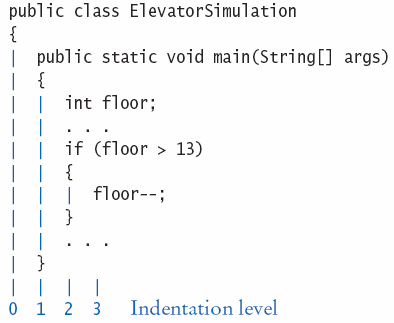
\includegraphics[height=0.45\paperheight,center]{pucrs-ep-fprog-unidade_03-decisoes-laminas-indentacao.png}
\end{figure}
\end{itemize}
\end{frame}

%-------------------------------------------------------
\begin{frame}[fragile]\frametitle{Erros Comuns}
\begin{itemize}
	\item Um erro comum é colocar um \texttt{;} depois do comando \texttt{if}:
\begin{javacode}
if (floor > 13) ;
{
   floor--;
}
\end{javacode}
	\item Um \texttt{;}, sem comando antes, é um \textbf{comando vazio}
	\item Portanto, no exemplo acima, o comando \texttt{if} \textbf{NÃO FARÁ NADA} se o teste for verdadeiro (comando vazio) e o bloco (entre chaves) será executado independentemente do teste
\end{itemize}
\end{frame}

%=======================================================
\section{Comparando Números}

%-------------------------------------------------------
\begin{frame}[fragile]\frametitle{Comparando Números}
\begin{itemize}
	\item Todo comando \texttt{if} tem uma condição que geralmente compara dois valores usando um operador
\begin{javacode}
if (floor > 13) ...
if (floor >= 13) ...
if (floor < 13) ...
if (floor <= 13) ...
if (floor == 13) ...
if (floor != 13) ...
\end{javacode}
\end{itemize}
\end{frame}

%-------------------------------------------------------
\begin{frame}[fragile]\frametitle{Operadores Relacionais}
\begin{center}
\begin{tikzpicture}
\node[drop shadow,fill=white,inner sep=0pt] 
{\rowcolors{1}{RoyalBlue!20}{RoyalBlue!5}
  \begin{tabular}{|c|c|c|}
\hline
    \textbf{Java} & \textbf{Notação Matemática} & \textbf{Descrição} \\
\hline
    \texttt{>}  & $>$ & Maior que \\
    \texttt{>=} & $\ge$ & Maior ou igual que \\
    \texttt{<}  & $<$ & Menor que \\
    \texttt{<=} & $\le$ & Menor ou igual que \\
    \texttt{==} & $=$ & Igual \\
    \texttt{!=} & $\neq$ & Diferente \\
\hline
  \end{tabular}
};
\end{tikzpicture}
\end{center}
\end{frame}

%-------------------------------------------------------
\begin{frame}[fragile]\frametitle{Precedência de Operadores}
\begin{itemize}
	\item Os operadores de comparação tem menor precedência do que operadores aritméticos
	\begin{itemize}
		\item Cálculos são feitos antes das comparações
		\item Normalmente os cálculos estão do lado direito de operadores de comparação ou atribuição
\begin{javacode}
actualFloor = floor + 1;
if (floor > height + 1) ...
\end{javacode}
	\end{itemize}
\end{itemize}
\end{frame}

%-------------------------------------------------------
\begin{frame}\frametitle{Exemplos de Operadores Relacionais (1)}
{\footnotesize
\begin{center}
\begin{tikzpicture}
\node[drop shadow,fill=white,inner sep=0pt] 
{\rowcolors{1}{RoyalBlue!20}{RoyalBlue!5}
  \begin{tabular}{|l|c|p{6cm}|}
\hline
\textbf{Expressão} & \textbf{Valor} & \textbf{Comentário} \\
\hline
\texttt{3 <= 4}     & \texttt{true}               & \texttt{3} é menor do que \texttt{4}; \texttt{<=} testa se é ``menor ou igual''.\\
\texttt{3 =< 4}     & \textcolor{red}{\textbf{X}} & O operador ``menor ou igual'' é \texttt{<=}, e não \texttt{=<}. O símbolo ``menor que'' vem antes.\\
\texttt{3 > 4}      & \texttt{false}              & \texttt{>} é o oposto de \texttt{<=}\\
\texttt{4 < 4}      & \texttt{false}              & O lado esquerdo da comparação tem que ser menor do que o lado direito.\\
\texttt{4 <= 4}     & \texttt{true}               & Ambos os lados são iguais; \texttt{<=} testa se é ``menor ou igual''\\
\texttt{3 == 5 - 2} & \texttt{true}               & \texttt{==} testa igualdade.\\
\texttt{3 != 5 - 1} & \texttt{true}               & \texttt{!=} testa diferença. É verdadeiro que \texttt{3} não é \texttt{5-1}.\\
\hline
  \end{tabular}
};
\end{tikzpicture}
\end{center}
}
\end{frame}

%-------------------------------------------------------
\begin{frame}\frametitle{Uso de Operadores Relacionais (2)}
{\footnotesize
\begin{center}
\begin{tikzpicture}
\node[drop shadow,fill=white,inner sep=0pt] 
{\rowcolors{1}{RoyalBlue!20}{RoyalBlue!5}
  \begin{tabular}{|l|c|p{6cm}|}
\hline
\textbf{Expressão} & \textbf{Valor} & \textbf{Comentário} \\
\hline
\texttt{3 = 6 / 2}  & \textcolor{red}{\textbf{X}} & Use \texttt{==} para testar igualdade.\\
\texttt{1.0 / 3.0 == 0.333333333} & \texttt{false} & Embora os valores sejam muito próximos um do outro, eles não são exatamente iguais.\\
\texttt{"10"} \texttt{> 5}   & \textcolor{red}{\textbf{X}} & Você não pode comparar um \emph{string} com um número.\\
\hline
  \end{tabular}
};
\end{tikzpicture}
\end{center}
}
\end{frame}

%-------------------------------------------------------
\begin{frame}[fragile]\frametitle{Erro Comum: Comparação de Números de Ponto-flutuante}
\begin{itemize}
	\item Números de ponto-flutuante tem precisão limitada
	\item Erros de arredondamento podem levar a resultados inesperados
{\small
\begin{javacode}
double r = Math.sqrt(2.0);
if (r*r == 2.0) {
   System.out.println("Math.sqrt(2.0) ao quadrado eh 2.0");
}
else {
   System.out.println("Math.sqrt(2.0) ao quadrado "+
                      "nao eh 2.0, mas "+r*r);   
}
\end{javacode}
}
	\item Resultado:
\begin{verbatim}
Math.sqrt(2.0) ao quadrado nao eh 2.0, mas 2.00000000000000044
\end{verbatim}
\end{itemize}
\end{frame}

%-------------------------------------------------------
\begin{frame}[fragile]\frametitle{O Uso de EPSILON}
\begin{itemize}
	\item Use um valor bastante pequeno para comparar se a diferença entre valores de ponto-flutuante está ``suficientemente perto''
	\begin{itemize}
		\item A magnitude da diferença entre os dois valores deve ser menor do que determinado limite
		\item Matematicamente, diz-se que x e y estão suficientemente próximos se $|x-y|<\varepsilon$
	\end{itemize}
\begin{javacode}
final double EPSILON = 1E-14;
double r = Math.sqrt(2.0);
if (Math.abs(r * r - 2.0) < EPSILON) {
   System.out.println("Math.sqrt(2.0) ao quadrado eh "+
                      "aproximadamente 2.0");
}
\end{javacode}
\end{itemize}
\end{frame}

%-------------------------------------------------------
\begin{frame}\frametitle{Implementando um Comando \texttt{if}}
\begin{itemize}
\item \textbf{Problema:} A livraria da Universidade realiza um Dia Kilobyte de Descontos sempre no dia 24 de outubro,
dando um desconto de 8\% em todos as compras de acessórios de computador se o preço for menor do que R\$128,00, e um
desconto de 16\% se o preço é no mínimo R\$128,00.
\end{itemize}
\end{frame}

%-------------------------------------------------------
\begin{frame}\frametitle{Implementando um Comando \texttt{if}}
\begin{itemize}
\item \textbf{Passos:}
	\begin{enumerate}
		\item Decida qual será a condição para decisão:\\ \texttt{preço original < 128?}
		\item Escreva o pseudocódigo para o ramo verdadeiro:\\ \texttt{preço com desconto = 0,92 x preço original}
		\item Escreva o pseudocódigo para o ramo falso:\\ \texttt{preço com desconto = 0,84 x preço original}
		\item Faça uma verificação dos operadores relacionais, testando-os com valores abaixo ($127$), igual ($128$) e acima ($129$)
		\item Remova a duplicação:\\ \texttt{preço com desconto = \_\_\_ x preço original}
		\item Teste ambos os ramos:\\ \texttt{preço com desconto = 0,92 x 100 = 92\\preço com desconto = 0,84 x 200 = 168}
		\item Escreva o código em Java
	\end{enumerate}
\end{itemize}
\end{frame}

%-------------------------------------------------------
\begin{frame}[fragile]\frametitle{Exemplo Implementado}
\begin{javacode}
if (precoOriginal < 128) {
   taxaDesconto = 0.92;
}
else {
   taxaDesconto = 0.84;
}
precoComDesconto = taxaDesconto * precoOriginal;
\end{javacode}
\end{frame}

%=======================================================
\section{Expressões condicionais}

%-------------------------------------------------------
\begin{frame}[fragile]\frametitle{O Operador Condicional}
\begin{itemize}
	\item Há uma forma abreviada de seleção que não é usada no livro-texto, mas que poderá aparecer em outros códigos
	\item Trata-se de uma atribuição com a seguinte sintaxe:\\
	{\tiny \texttt{variável = condição ? expressão\_para\_condição\_verdadeira : expressão\_para\_condição\_falsa ;}}
	\item Por exemplo:
\begin{javacode}
actualFloor = floor > 13 ? floor - 1 : floor;
\end{javacode}
	\item Nesta forma abreviada aparecem todas as partes de um \texttt{if-else}, porém usando:
	\begin{itemize}
		\item \texttt{?} para inciar o ramo verdadeiro e
		\item \texttt{:} para iniciar o ramo falso
	\end{itemize}
\end{itemize}
\end{frame}

%-------------------------------------------------------
\begin{frame}[fragile]\frametitle{Exemplos}
\begin{javacode}
// Exemplo 1
int inteiro = in.nextInt();
System.out.println( (inteiro%2 == 0) ? "Par" : "Impar" );

// Exemplo 2
taxaDesconto = (preco < 128) ? 0.92 : 0.84;
precoComDesconto = taxaDesconto * preco;

// OU

precoComDesconto = ( (preco < 128) ? 0.92 : 0.84 ) * preco;
\end{javacode}
\end{frame}

%=======================================================
\section{Comparando Strings}

%-------------------------------------------------------
\begin{frame}[fragile]\frametitle{Comparando \emph{Strings}}
\begin{itemize}
	\item \emph{Strings} são um pouco ``especiais'' em Java
	\item Não use o operador \texttt{==} com \emph{strings}
	\begin{itemize}
		\item O seguinte trecho funciona, mas na verdade compara a localização de duas \emph{strings} e não os seus conteúdos
\begin{javacode}
if (string1 == string2) ...
\end{javacode}
		\item Em vez disto uso o método \texttt{equals}:
\begin{javacode}
if (string1.equals(string2)) ...
\end{javacode}
	\end{itemize}
\end{itemize}
\end{frame}

%-------------------------------------------------------
\begin{frame}[fragile]\frametitle{Exemplos}

\begin{javacode}
if ( "Tomate".substring(0,3).equals("Tom") )
   System.out.println( ">>> true <<<" );
else
   System.out.println( "false" );

if ( "Tomate".substring(0,3) == ("Tom") )
   System.out.println( "true" );
else
   System.out.println( ">>> false <<<" );
\end{javacode}
\end{frame}

%-------------------------------------------------------
\begin{frame}[fragile]\frametitle{Mais um exemplo}
\begin{itemize}
	\item Java cria uma nova variável \texttt{String} cada vez que é usado um texto entre aspas
	\item Se há uma \emph{string} que coincida exatamente com ela, Java a reusa
\footnotesize{
\begin{javacode}
String nickname = "Rob";
if (nickname == "Rob")
   System.out.println( ">>> true <<<" );
else
   System.out.println( "false" );
\end{javacode}
\begin{javacode}
String name = "Robert";
String nickname = name.substring(0,3);
if (nickname == "Rob")
   System.out.println( "true" );
else
   System.out.println( ">>> false <<<" );
\end{javacode}
}
\end{itemize}
\end{frame}

%-------------------------------------------------------
\begin{frame}\frametitle{Ordem Lexicográfica}
\begin{itemize}
	\item Para comparar \emph{strings} pela ordem de dicionário, pode-se usar \texttt{compareTo()}
	\item Considerando duas \emph{strings} \texttt{string1} e \texttt{string2}:
	\begin{itemize}
		\item \texttt{string1.compareTo(string2)} será \textbf{menor do que zero} se \texttt{string1} vier antes de \texttt{string2}
		\item \texttt{string1.compareTo(string2)} será \textbf{igual a zero} se elas forem iguais
		\item \texttt{string1.compareTo(string2)} será \textbf{maior do que zero} se \texttt{string1} vier depois de \texttt{string2}
	\end{itemize}
	\item Observações:
	\begin{itemize}
		\item Todas as letras maiúsculas vem antes das minúsculas
		\item ``Espaço'' vem antes de todos os caracteres imprimíveis
		\item Dígitos (0-9) vem antes das letras
	\end{itemize}
	\item Lembre-se: para comparar desconsiderando a diferença entre minúsculas e maiúsculas, pode-se usar \texttt{equalsIgnoreCase} e \texttt{compareToIgnoreCase}
\end{itemize}
\end{frame}

%=======================================================
\section{Múltiplas Alternativas}

%-------------------------------------------------------
\begin{frame}\frametitle{Múltiplas Alternativas}
\begin{itemize}
	\item Um \texttt{if} tem 2 ramos, mas o que acontece se forem necessários mais do que dois ramos?
	\item Por exemplo, uma escala para o efeito de um terremoto:
	\begin{itemize}
		\item 8 (ou mais): a maioria das edificações cai
		\item 7 to 7.99: muitas edificações destruídas
		\item 6 to 6.99: muitas edificações bastante danificadas, algumas desmoronadas
		\item 4.5 to 5.99: danos a edificações mal construídas
		\item menos do que 4.5: nenhuma edificação destruída
	\end{itemize}
\end{itemize}
\end{frame}

%-------------------------------------------------------
\begin{frame}\frametitle{Fluxograma para Múltiplos Ramos}
\begin{figure}[h]
	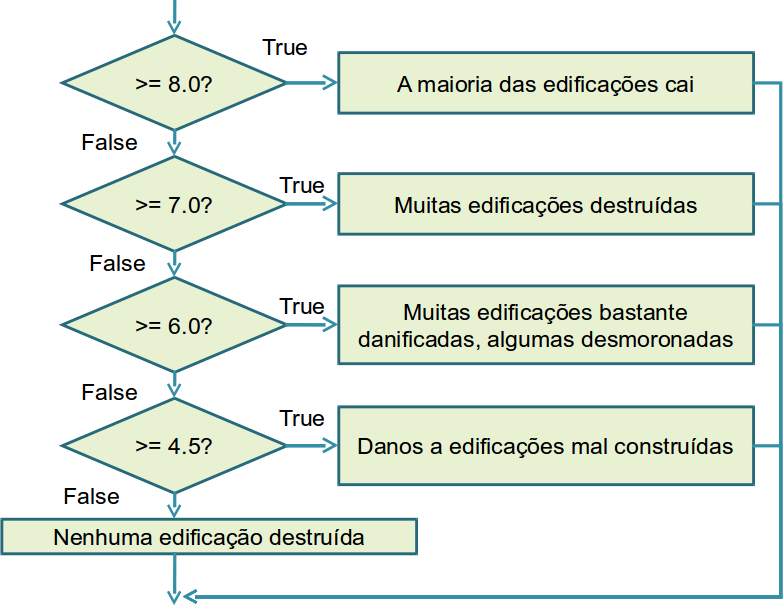
\includegraphics[height=0.7\paperheight,center]{pucrs-ep-fprog-unidade_03-decisoes-laminas-fluxograma_multiplos_ramos.png}
\end{figure}
\end{frame}

%-------------------------------------------------------
\begin{frame}[fragile]\frametitle{O que há de errado com este código?}
{\footnotesize
\begin{javacode}
if (richter >= 8.0) {
  System.out.println("A maioria das edificacoes cai");
}
if (richter >= 7.0) {
  System.out.println("Muitas edificacoes destruidas");
}
if (richter >= 6.0) {
  System.out.println("Muitas edificacoes bastante danificadas, "+
                     "algumas desmoronadas");
}
if (richter >= 4.5) {
  System.out.println("Danos a edificacoes mal construidas");
}
if (richter < 4.5) {
  System.out.println("Nenhuma edificacao destruida");
}
\end{javacode}
}
\end{frame}

%-------------------------------------------------------
\begin{frame}[fragile]\frametitle{E com este código? O que há de errado?}
{\footnotesize
\begin{javacode}
if (richter >= 8.0) {
   System.out.println("A maioria das edificacoes cai");
}
if (richter < 8.0 && richter >= 7.0) {
   System.out.println("Muitas edificacoes destruidas");
}
if (richter < 7.0 && richter >= 6.0) {
   System.out.println("Muitas edificacoes bastante danificadas, "+
                      "algumas desmoronadas");
}
if (richter < 6.0 && richter >= 4.5) {
   System.out.println("Danos a edificacoes mal construidas");
}
if (richter < 4.5) {
   System.out.println("Nenhuma edificacao destruida");
}
\end{javacode}
}
\end{frame}

%-------------------------------------------------------
\begin{frame}[fragile]\frametitle{Construção \texttt{if-else-if}}
{\footnotesize
\begin{javacode}
if (richter >= 8.0) {
   System.out.println("A maioria das edificacoes cai");
}
else if (richter >= 7.0) {
   System.out.println("Muitas edificacoes destruidas");
}
else if (richter >= 6.0) {
   System.out.println("Muitas edificacoes bastante danificadas, "+
                      "algumas desmoronadas");
}
else if (richter >= 4.5) {
   System.out.println("Danos a edificacoes mal construidas");
}
else {
   System.out.println("Nenhuma edificacao destruida");
}
\end{javacode}
}
\end{frame}

%-------------------------------------------------------
\begin{frame}\frametitle{Exercício}
\begin{enumerate}
	\item Escreva um programa em Java que leia dois valores reais, \texttt{x} e \texttt{y}, que correspondem às coordenadas de um ponto no plano cartesiano. E imprima em que quadrante este ponto se encontra (``1o. Quadrante'', ``2o. Quadrante'', ``3o. Quadrante'', ``4o. Quadrante'') ou se ele se encontra na origem (``Origem'') ou sobre um dos eixos (``Eixo X'', ``Eixo Y'').\\
Em um primeiro momento use os comandos \texttt{if} e \texttt{else}. Depois reescreva o programa usando expressões condicionais.
\end{enumerate}
\end{frame}

%-------------------------------------------------------
\begin{frame}\frametitle{Outra forma de Implementar Múltiplos Ramos}
\begin{itemize}
	\item O comando \texttt{switch} escolhe uma opção de um conjunto de opções
	\item Ele funciona com os tipos primitivos \texttt{byte}, \texttt{short}, \texttt{char} e \texttt{int}
	\item Também funciona com enumerações, a classe \texttt{String} e algumas outras classes (\texttt{Character}, \texttt{Byte}, \texttt{Short} e \texttt{Integer}) que podem ser convertidas para os tipos primitivos suportados
	\item O comando \texttt{break} encerra cada \texttt{case}
	\item \texttt{default} trata todas as opções não indicadas nos \texttt{case}s
\end{itemize}
\end{frame}

%-------------------------------------------------------
\begin{frame}[fragile]\frametitle{Exemplo de \texttt{switch}/\texttt{case}}
\begin{javacode}
int digit = ...;
switch (digit) {
  case 1: digitName = "one";   break;
  case 2: digitName = "two";   break;
  case 3: digitName = "three"; break;
  case 4: digitName = "four";  break;
  case 5: digitName = "five";  break;
  case 6: digitName = "six";   break;
  case 7: digitName = "seven"; break;
  case 8: digitName = "eight"; break;
  case 9: digitName = "nine";  break;
  default: digitName = "";     break;
}
\end{javacode}
\end{frame}

%=======================================================
\section{Decisões Aninhadas}

%-------------------------------------------------------
\begin{frame}\frametitle{Decisões Aninhadas}
\begin{itemize}
	\item Você pode aninhar um \texttt{if} dentro de um ramo de um comando \texttt{if}
	\item Um exemplo simples: pedidos de bebidas em um bar
	\begin{itemize}
		\item Pergunte ao cliente o que ele quer beber
		\item Se o cliente pedir vinho:
		\begin{itemize}
			\item Peça a identidade do cliente
			\item Se a idade do cliente for maior ou igual a 21, então\\Sirva vinho
			\item Senão\\Polidamente explique como funciona a lei ao cliente 
		\end{itemize}
		\item Senão
		\begin{itemize}
			\item Sirva uma bebida não alcoólica ao cliente
		\end{itemize}
	\end{itemize}
\end{itemize}
\end{frame}

%-------------------------------------------------------
\begin{frame}\frametitle{Fluxograma de um \texttt{if} aninhado}
\begin{figure}[h]
	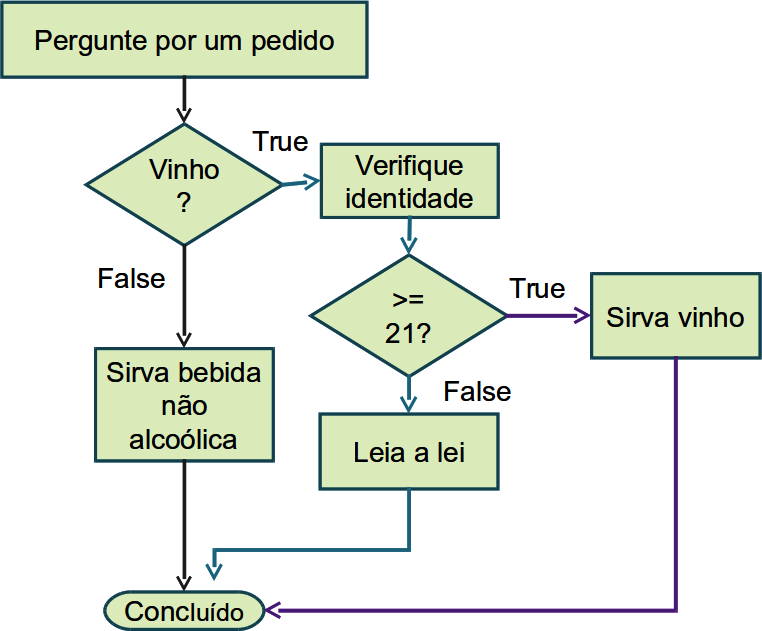
\includegraphics[height=0.65\paperheight,center]{pucrs-ep-fprog-unidade_03-decisoes-laminas-fluxograma_bebida.png}
\end{figure}
\begin{center}
{\tiny \texttt{if-else} aninhado dentro do ramo verdadeiro de um comando \texttt{if}: 3 partes}
\end{center}
\end{frame}

%-------------------------------------------------------
\begin{frame}\frametitle{Acompanhamento Manual (ou Teste de Mesa)}
\begin{itemize}
	\item Acompanhar a execução manualmente ajuda a entender se o programa está funcionando corretamente ou não
	\item Crie uma tabela com as variáveis mais importantes
	\begin{itemize}
		\item Use lápis e papel para acompanhar os valores destas variáveis
	\end{itemize}
	\item Pode ser feito com pseudocódigo ou até mesmo código Java
	\begin{itemize}
		\item Você pode marcar a execução no código com um \emph{clips}
	\end{itemize}
	\item Use valores de entrada:
	\begin{itemize}
		\item Para os quais você já sabe os resultados que serão produzidos
		\item Que testem todos os ramos possíveis do seu código 
	\end{itemize}
\end{itemize}
\end{frame}

%-------------------------------------------------------
\begin{frame}\frametitle{Teste de Mesa para o programa \texttt{TaxCalculator.java}}
\begin{itemize}
	\item Monte uma tabela para anotar os valores das variáveis
\begin{figure}[h]
	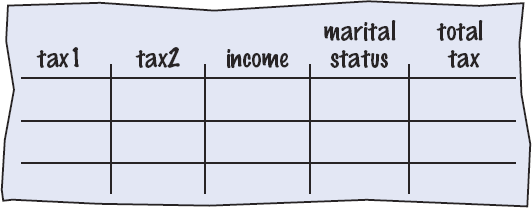
\includegraphics[height=0.30\paperheight,center]{pucrs-ep-fprog-unidade_03-decisoes-laminas-tabela.png}
\end{figure}
	\item Teste com as seguintes entradas
	\begin{itemize}
		\item \texttt{income=20000, maritalStatus="s"}
		\item \texttt{income=40000, maritalStatus="s"}
		\item \texttt{income=40000, maritalStatus="m"}
		\item \texttt{income=80000, maritalStatus="m"}
	\end{itemize}
\end{itemize}
\end{frame}

%-------------------------------------------------------
\begin{frame}[fragile]\frametitle{Erro Comum: \texttt{else} ``desamparado''}
\begin{itemize}
	\item Quando um \texttt{if} é aninhado dentro de outro \texttt{if}, o seguinte pode ocorrer:
\begin{javacode}
double shippingCharge = 5.00; // $5 inside continental U.S.
if (country.equals("USA"))
  if (state.equals("HI"))
    shippingCharge = 10.00;   // Hawaii is more expensive
else // Pitfall!
  shippingCharge = 20.00;     // As are foreign shipment
\end{javacode}
	\item O nível de indentação sugere que o \texttt{else} esteja relacionado ao \texttt{if} de \texttt{country.equals("USA")}
	\item Porém a cláusula \texttt{else} sempre se associa ao \texttt{if} mais próximo
\end{itemize}
\end{frame}

%-------------------------------------------------------
\begin{frame}[fragile]\frametitle{Tipos Enumerados}
Java provê uma forma simples de nomear uma lista finita de valores que uma variável pode armazenar
\begin{itemize}
	\item Funciona como uma declaração de novos tipos, com uma lista de possíveis valores
{\scriptsize
\begin{javacode}
public enum FilingStatus { 
 SINGLE, MARRIED,MARRIED_FILING_SEPARATELY
}
\end{javacode}
}
	\item Você pode ter qualquer número de valores, mas tem que incluir eles todos na declaração \texttt{enum}
	\item Você pode declarar variáveis do tipo ``enumeração''
{\scriptsize
\begin{javacode}
FilingStatus status = FilingStatus.SINGLE;
\end{javacode}
}
	\item Você também pode usar o operador de comparação entre eles:
{\scriptsize
\begin{javacode}
if (status == FilingStatus.SINGLE) ... 
\end{javacode}
}
\end{itemize}
\end{frame}

%=======================================================
\section{Solução de Problemas: Casos de Teste}

%-------------------------------------------------------
\begin{frame}\frametitle{Solução de Problemas: Casos de Teste}
\begin{itemize}
	\item Procure fazer uma cobertura completa de todos os pontos de decisão
	\begin{itemize}
		\item Todos os ramos do seu código devem ser cobertos por um caso de teste
		\item Por exemplo, há duas possibilidades para o estado civil e duas possibilidades de taxa, levando a $4$ casos de teste
		\item Teste vários valores de limite (valores que são testados no seu código), tais como uma renda que esteja entre as duas possibilidades, e uma renda igual a zero
		\item Se você estiver responsável pela verificação de erro, também teste entradas inválidas, tais como rendas negativas
	\end{itemize}
\end{itemize}
\end{frame}

%-------------------------------------------------------
\begin{frame}\frametitle{Casos de Teste para o Cálculo de Taxas}
\begin{itemize}
	\item Escolha valores de entrada que testem limites e valores nulos e também teste cada ramo do código
\begin{center}
\begin{tikzpicture}
\node[drop shadow,fill=white,inner sep=0pt] 
{\rowcolors{1}{RoyalBlue!20}{RoyalBlue!5}
  \begin{tabular}{|c|c|c|}
\hline
    \textbf{Caso de Teste} & \textbf{Saída Esperada} & \textbf{Comentário} \\
\hline
    \texttt{30.000 ~ s}  & \texttt{3.000} & Taxa de 10\% \\
    \texttt{72.000 ~ s}  & \texttt{13.200} & 3.200 + 25\% de 40.000 \\
    \texttt{50.000 ~ m}  & \texttt{5.000} & Taxa de 10\% \\
    \texttt{104.000 ~ m}  & \texttt{16.400} & 6.400 + 25\% de 40.000 \\
    \texttt{32.000 ~ m}  & \texttt{3.200} & Caso limite \\
    \texttt{0}  & \texttt{0} & Caso limite \\
\hline
  \end{tabular}
};
\end{tikzpicture}
\end{center}
\end{itemize}
\end{frame}

%=======================================================
\section{Variáveis e operadores Booleanos}

%-------------------------------------------------------
\begin{frame}[fragile]\frametitle{Variáveis e operadores Booleanos}
\begin{itemize}
	\item Variáveis Booleanas
	\begin{itemize}
		\item Uma variável booleana é frequentemente chamada de \emph{flag} porque pode assumir ou o valor verdadeiro (\emph{true}) ou falso (\emph{false})
		\item Java dispõe do tipo \texttt{boolean} para variáveis booleanas, que podem assumir ou \texttt{true} ou \texttt{false}
\begin{javacode}
boolean acertou = true;
boolean sair = false;
\end{javacode}
	\end{itemize}
	\item Operadores Booleanos: \texttt{\&\&} e \texttt{||}
	\begin{itemize}
		\item São usados para combinar múltiplas condições
		\item \texttt{\&\&} é o operador AND (E)
		\item \texttt{||} é o operador OR (OU)
	\end{itemize}
\end{itemize}
\end{frame}

%-------------------------------------------------------
\begin{frame}[fragile]\frametitle{Condições Combinadas: \texttt{\&\&}}
\begin{itemize}
	\item A combinação de dois testes ou condições é usada frequentemente para verificar se um valor está dentro de um intervalo
	\item Ambos os lados do AND devem ser verdadeiros para que o resultado também seja:
{\scriptsize
\begin{javacode}
if (temp > 0 && temp < 100) {
  System.out.println("Liquido"); 
}
\end{javacode}
}
\end{itemize}
\begin{figure}[h]
	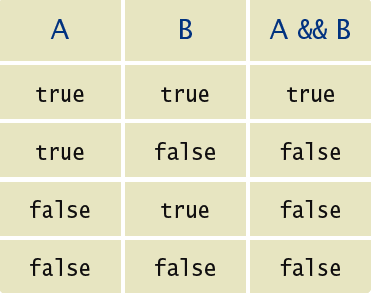
\includegraphics[height=0.35\paperheight,center]{pucrs-ep-fprog-unidade_03-decisoes-laminas-and.png}
\end{figure}
\end{frame}

%-------------------------------------------------------
\begin{frame}[fragile]\frametitle{Condições Combinadas: \texttt{||}}
\begin{itemize}
	\item Se apenas um dos testes precisa ser verdadeiro, pode-se combinar os testes com OR
	\item Se um dos lados do OR for verdadeiro, o resultado também será:
{\scriptsize
\begin{javacode}
if (balance > 100 || credit > 100) {
  System.out.println("Aceito"); 
}
\end{javacode}
}
\end{itemize}
\begin{figure}[h]
	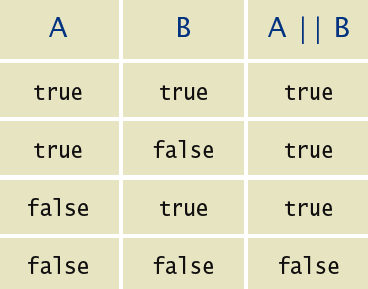
\includegraphics[height=0.35\paperheight,center]{pucrs-ep-fprog-unidade_03-decisoes-laminas-or.png}
\end{figure}
\end{frame}

%-------------------------------------------------------
\begin{frame}[fragile]\frametitle{O Operador NOT: \texttt{!}}
\begin{itemize}
	\item Se for necessário inverter o valor de uma variável booleana ou de uma condição, basta precedê-la com \texttt{!}:
\begin{figure}[h]
	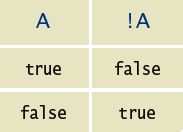
\includegraphics[height=0.15\paperheight,center]{pucrs-ep-fprog-unidade_03-decisoes-laminas-not.png}
\end{figure}
	\item O que é melhor?
\begin{columns}
\begin{column}{0.5\linewidth}
{\footnotesize
\begin{javacode}
if (!attending || grade < 60)
   System.out.println("Drop?"); 
\end{javacode}
}
\end{column}
\begin{column}{0.5\linewidth}
{\footnotesize
\begin{javacode}
if (attending && !(grade < 60))
   System.out.println("Stay"); 
\end{javacode}
}
\end{column}
\end{columns}
	\item Ao usar \texttt{!}, procure simplificar a lógica:
{\footnotesize
\begin{javacode}
if (attending && grade >= 60) ...
\end{javacode}
}
\end{itemize}
\end{frame}

%-------------------------------------------------------
\begin{frame}[fragile]\frametitle{Fluxograma para AND}
\begin{itemize}
	\item Isto é frequentemente chamado de ``verificação de limite'', sendo usado para validar se uma entrada está entre 2 valores
\begin{javacode}
if (temp > 0 && temp < 100) {
  System.out.println("Liquid"); 
}
\end{javacode}
\end{itemize}
\end{frame}

%-------------------------------------------------------
\begin{frame}[fragile]\frametitle{Fluxograma para AND}
\begin{figure}[h]
	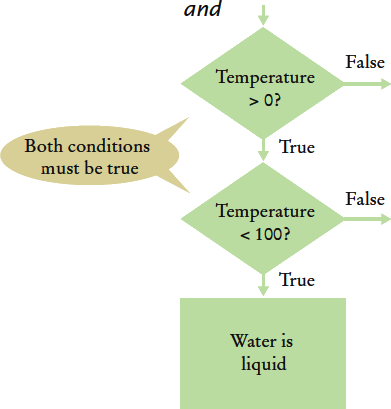
\includegraphics[height=0.70\paperheight,center]{pucrs-ep-fprog-unidade_03-decisoes-laminas-fluxograma_and.png}
\end{figure}
\end{frame}

%-------------------------------------------------------
\begin{frame}[fragile]\frametitle{Fluxograma para OR}
\begin{itemize}
	\item Outra forma de ``verificação de limite'': verifica se o valor está fora do limite
\begin{javacode}
if (temp <= 0 || temp >= 100) {
  System.out.println("Not Liquid"); 
}
\end{javacode}
\end{itemize}
\end{frame}

%-------------------------------------------------------
\begin{frame}[fragile]\frametitle{Fluxograma para OR}
\begin{figure}[h]
	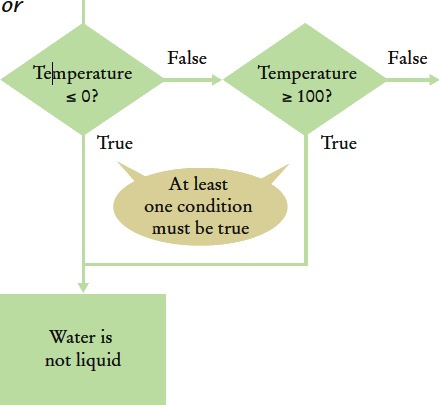
\includegraphics[height=0.70\paperheight,center]{pucrs-ep-fprog-unidade_03-decisoes-laminas-fluxograma_or.png}
\end{figure}
\end{frame}

%-------------------------------------------------------
\begin{frame}\frametitle{Exemplos de Uso de Operadores Booleanos (1)}
{\small
\begin{center}
\begin{tikzpicture}
\node[drop shadow,fill=white,inner sep=0pt] 
{\rowcolors{1}{RoyalBlue!20}{RoyalBlue!5}
  \begin{tabular}{|p{4.5cm}|p{3.5cm}|p{6cm}|}
\hline
    \textbf{Expressão} & \textbf{Valor} & \textbf{Comentário}\\
\hline
    \texttt{0 < 200 \&\& 200 < 100}       & \texttt{false}    & Apenas a primeira condição é verdadeira.\\
    \texttt{0 < 200 || 200 < 100}       & \texttt{true}     & A primeira condição é verdadeira.\\
    \texttt{0 < 200 || 100 < 200}       & \texttt{true}     & O operador \texttt{||} não é um operador para ``ou-ou''. Se ambas as condições são verdadeiras, o resultado é verdadeiro.\\
    \texttt{0 < x \&\& x < 100 || x == -1}       & \texttt{(0 < x \&\& x < 100) || x == -1}    & O operador \texttt{\&\&} tem maior precedência que o operador \texttt{||}.\\
    \texttt{0 < x < 100}          &  \textcolor{red}{\textbf{ERRO}}   & \textbf{Erro:} Esta expressão não testa se \texttt{x} está entre 0 e 100. A expressão \texttt{0 < x} gera um valor booleano, que não pode ser comparado com o valor inteiro 100.\\
\hline
  \end{tabular}
};
\end{tikzpicture}
\end{center}
}
\end{frame}

%-------------------------------------------------------
\begin{frame}\frametitle{Exemplos de Uso de Operadores Booleanos (2)}
{\small
\begin{center}
\begin{tikzpicture}
\node[drop shadow,fill=white,inner sep=0pt] 
{\rowcolors{1}{RoyalBlue!20}{RoyalBlue!5}
  \begin{tabular}{|p{5cm}|p{3cm}|p{6cm}|}
\hline
    \textbf{Expressão} & \textbf{Valor} & \textbf{Comentário}\\
\hline
    \texttt{x \&\& y > 0}          &  \textcolor{red}{\textbf{ERRO}}   & \textbf{Erro:} Esta expressão não testa se \texttt{x} e \texttt{y} são ambos positivos. A parte à direita de \texttt{\&\&} é um inteiro (\texttt{x}) e a parte direita é um booleando (\texttt{y > 0}). Não se pode usar \texttt{\&\&} com um valor inteiro.\\
    \texttt{!(0 < 200)}       & \texttt{false}     & \texttt{0 < 200} é verdadeiro, portanto, a sua negação é falsa.\\
    \texttt{frozen == true}       & \texttt{frozen}     & Não é necessário comparar uma variável booleana com \texttt{true}.\\
    \texttt{frozen == false}       & \texttt{!frozen}     & É mais claro usar \texttt{!} do que comparar com \texttt{false}.\\
\hline
  \end{tabular}
};
\end{tikzpicture}
\end{center}
}
\end{frame}

%-------------------------------------------------------
\begin{frame}[fragile]\frametitle{Erros Comuns (1)}
\begin{itemize}
	\item Combinação de múltiplos operadores relacionais
	\begin{itemize}
		\item O seguinte formato é usado na matemática, mas não em Java:
\begin{javacode}
if (0 <= temp <= 100)  // Erro de sintaxe!
\end{javacode}
		\item São necessárias duas comparações:
\begin{javacode}
if (0 <= temp && temp <= 100) 
\end{javacode}
	\end{itemize}
	\item Isto também não é permitido em Java:
\begin{javacode}
if (input == 1 || 2)  // Erro de sintaxe!
\end{javacode}
	\begin{itemize}
		\item Isto também exige 2 comparações:
\begin{javacode}
if (input == 1 || input == 2)
\end{javacode}
	\end{itemize}
\end{itemize}
\end{frame}

%-------------------------------------------------------
\begin{frame}[fragile]\frametitle{Erros Comuns (2)}
Confundir condições \texttt{\&\&} e \texttt{||}
\begin{itemize}
	\item É um erro surpreendentemente comum confundir condições \texttt{\&\&} e \texttt{||}
	\item Se um valor está no intervalo de 0 a 100, ele é no mínimo 0 \textbf{e} no máximo 100
	\item Se ele está fora deste intervalo, ele é menor do que 0 \textbf{ou} maior do que 100
	\item Não há nenhuma regra de mágica; basta pensar com cuidado
\end{itemize}
\end{frame}


%-------------------------------------------------------
\begin{frame}[fragile]\frametitle{Avaliação \emph{short-circuit}: \texttt{\&\&}}
\begin{itemize}
	\item Condições combinadas são avaliadas da esquerda para a direita
	\item Se uma das condições avaliadas for falsa, por que continuar avaliando as demais?
\begin{javacode}
if (temp > 0 && temp < 100) {
  System.out.println("Liquid"); 
}
\end{javacode}
	\item Um exemplo útil:
\begin{javacode}
if (quantity > 0 && price / quantity < 10)
\end{javacode}
\end{itemize}
\end{frame}

%-------------------------------------------------------
\begin{frame}\frametitle{Avaliação \emph{short-circuit}: \texttt{\&\&}}
\begin{figure}[h]
	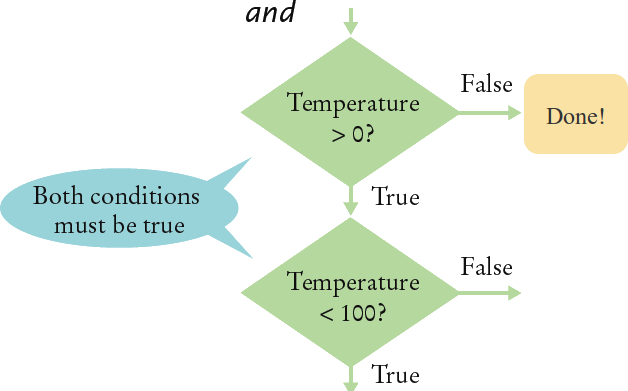
\includegraphics[height=0.70\paperheight,center]{pucrs-ep-fprog-unidade_03-decisoes-laminas-short_and.png}
\end{figure}
\end{frame}

%-------------------------------------------------------
\begin{frame}[fragile]\frametitle{Avaliação \emph{short-circuit}: \texttt{||}}
\begin{itemize}
	\item Se alguma condição à esquerda for verdadeira, por que continuar avaliando as demais?
\begin{javacode}
if (temp <= 0 || temp >= 100) {
  System.out.println("Not Liquid"); 
}
\end{javacode}
\end{itemize}
\end{frame}

%-------------------------------------------------------
\begin{frame}\frametitle{Avaliação \emph{short-circuit}: \texttt{||}}
\begin{figure}[h]
	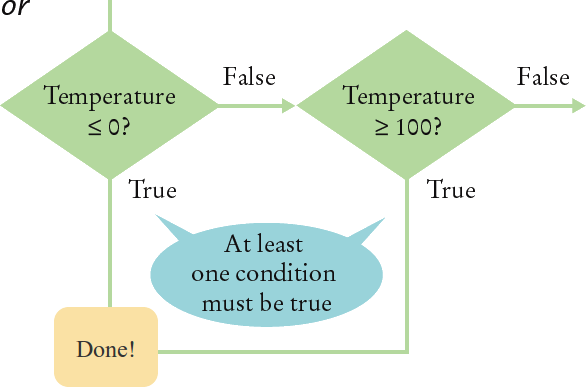
\includegraphics[height=0.70\paperheight,center]{pucrs-ep-fprog-unidade_03-decisoes-laminas-short_or.png}
\end{figure}
\end{frame}

%-------------------------------------------------------
\begin{frame}[fragile]\frametitle{Lei de De Morgan}
\begin{itemize}
	\item A Lei de De Morgan diz como negar condições \texttt{\&\&} e \texttt{||}
	\begin{itemize}
		\item \texttt{!(A \&\& B)} é o mesmo que \texttt{!A || !B}
		\item \texttt{!(A || B)} é o mesmo que \texttt{!A \&\& !B}
	\end{itemize}
	\item Exemplo: Envio para AK e HI é mais caro
{\scriptsize
\begin{javacode}
if ( !(country.equals("USA") && !state.equals("AK") && !state.equals("HI")) )
   shippingCharge = 20.00;
\end{javacode}
\begin{javacode}
if ( !country.equals("USA") || state.equals("AK") || state.equals("HI") )
   shippingCharge = 20.00;
\end{javacode}
}
	\item Para simplificar condições com negações de condições AND ou OR, geralmente é uma boa ideia aplicar a Lei de De Morgan para mover as negações para o nível mais interno.
\end{itemize}
\end{frame}

%=======================================================
\section{Aplicação: Validação da Entrada}

%-------------------------------------------------------
\begin{frame}[fragile]\frametitle{Aplicação: Validação da Entrada}
\begin{itemize}
	\item Aceitar entrada do usuário é perigoso
	\item Considere, por exemplo, o programa do elevador
	\begin{itemize}
		\item O usuário pode fornecer um caracter ou valor inválido
		\item Ele deveria fornecer um valor inteiro
		\item O método \texttt{hasNextInt} da classe Scanner pode ajudar: ele retorna \texttt{true} se o valor for um inteiro válido, ou \texttt{false} em caso contrário
		\item Depois pode-se verificar o intervalo do andar fornecido: deve estar entre $1$ e $20$; não deve ser $0$, nem $13$, nem $>20$
\begin{javacode}
if (in.hasNextInt()) {
  int floor = in.nextInt();
  // Process the input value
}
else {
  System.out.println("Not integer.");
}
\end{javacode}
	\end{itemize}
\end{itemize}
\end{frame}

%-------------------------------------------------------
\begin{frame}[fragile]\frametitle{\texttt{ElevatorSimulation2.java} (Parte 1)}
{\tiny
\begin{javacode}
import java.util.Scanner;

/**
   This program simulates an elevator panel that skips the 13th floor, checking for
   input errors.
 */
public class ElevatorSimulation2 {
   public static void main(String[] args) {
      Scanner in = new Scanner(System.in);
      System.out.print("Floor: ");
      if (in.hasNextInt()) {
         // Now we know that the user entered an integer
         int floor = in.nextInt();
         if (floor == 13) {
            System.out.println("Error: There is no thirteenth floor.");
         }
         else if (floor <= 0 || floor > 20) {
            System.out.println("Error: The floor must be between 1 and 20.");
         }
         else {
\end{javacode}
}
\end{frame}

%-------------------------------------------------------
\begin{frame}[fragile]\frametitle{\texttt{ElevatorSimulation2.java} (Parte 2)}
{\tiny
\begin{javacode}
            // Now we know that the input is valid
            int actualFloor = floor;
            if (floor > 13) {
               actualFloor = floor - 1;
            }
            System.out.println("The elevator will travel to the actual floor "
            + actualFloor);
         }
      }
      else {
         System.out.println("Error: Not an integer.");
      }
   }
}
\end{javacode}
}
\end{frame}

%-------------------------------------------------------
\begin{frame}[fragile]\frametitle{Métodos para Teste de Caracteres}
\begin{itemize}
	\item A classe \texttt{Character} tem um bom número de métodos que retornam o tipo \texttt{boolean}:
\begin{javacode}
if (Character.isDigit(ch)) {
  ...
}
\end{javacode}
\end{itemize}
\begin{center}
\begin{tikzpicture}
\node[drop shadow,fill=white,inner sep=0pt] 
{\rowcolors{1}{RoyalBlue!20}{RoyalBlue!5}
  \begin{tabular}{|c|c|}
\hline
    \textbf{Método} & \textbf{Exemplo de Caracteres Aceitos} \\
\hline
    \texttt{isDigit}  & 0, 1, 2 \\
    \texttt{isLetter}  & A, B, C, a, b, c \\
    \texttt{isUpperCase}  & A, B, C \\
    \texttt{isLowerCase}  & a, b, c \\
    \texttt{isWhiteSpace}  & espaço, nova linha, tabulação \\
\hline
  \end{tabular}
};
\end{tikzpicture}
\end{center}
\end{frame}

%=======================================================
\section{Exemplos}

%-------------------------------------------------------
\begin{frame}\frametitle{Custo de Postagem nos EUA: descrição e fluxograma}
\begin{itemize}
	\item O custo de envio interno nos EUA é de \$5, exceto para Hawaii e Alaska para onde o custo é de \$10. O custo internacional é de \$20.
\begin{figure}[h]
	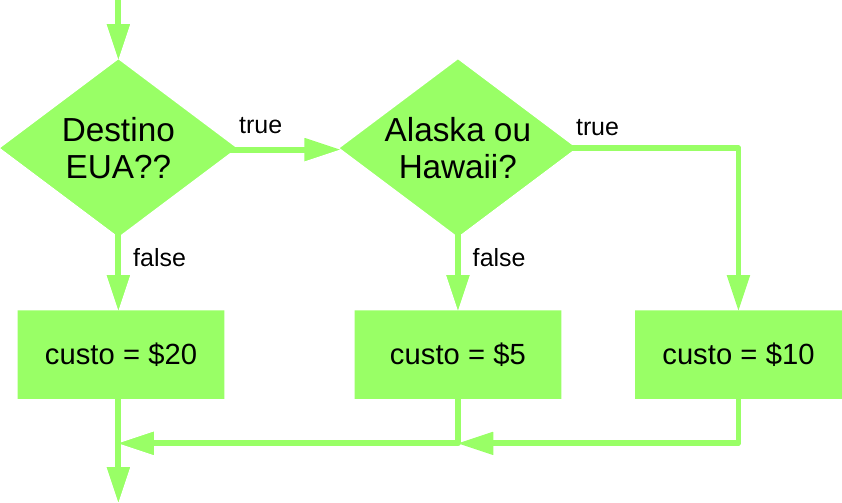
\includegraphics[height=0.50\paperheight,center]{pucrs-ep-fprog-unidade_03-decisoes-laminas-fluxograma_postagem_eua.png}
\end{figure}
\end{itemize}
\end{frame}

%-------------------------------------------------------
\begin{frame}[fragile]\frametitle{Custo de Postagem nos EUA: implementação}
\tiny{\inputminted[bgcolor=cyan!10]{java}{src/PostagemEUA.java}}		
\end{frame}

%-------------------------------------------------------
\begin{frame}\frametitle{Imposto de Renda nos EUA: descrição}
O imposto de renda anual nos EUA considera basicamente 2 alternativas iniciais: contribuição para solteiros e contribuição para casados.
Para cada uma destas possibilidades o imposto é calculado de forma diferente, conforme o ganho individual ou do casal.
\begin{itemize}
	\item Solteiro
	\begin{itemize}
		\item Renda menor ou igual a \$32.000,00\\
		taxa = 10\%
		\item Renda maior do que \$32.000,00\\
		taxa = \$3.200,00 + 25\% sobre o que exceder \$32.000,00
	\end{itemize}
	\item Casado
	\begin{itemize}
		\item Renda conjunta menor ou igual a \$64.000,00\\
		taxa = 10\%
		\item Renda conjunta maior do que \$64.000,00\\
		taxa = \$6.400,00 + 25\% sobre o que exceder \$64.000,00
	\end{itemize}
\end{itemize}
\end{frame}

%-------------------------------------------------------
\begin{frame}\frametitle{Imposto de Renda nos EUA: fluxograma}
\begin{center}
\begin{figure}[h]
	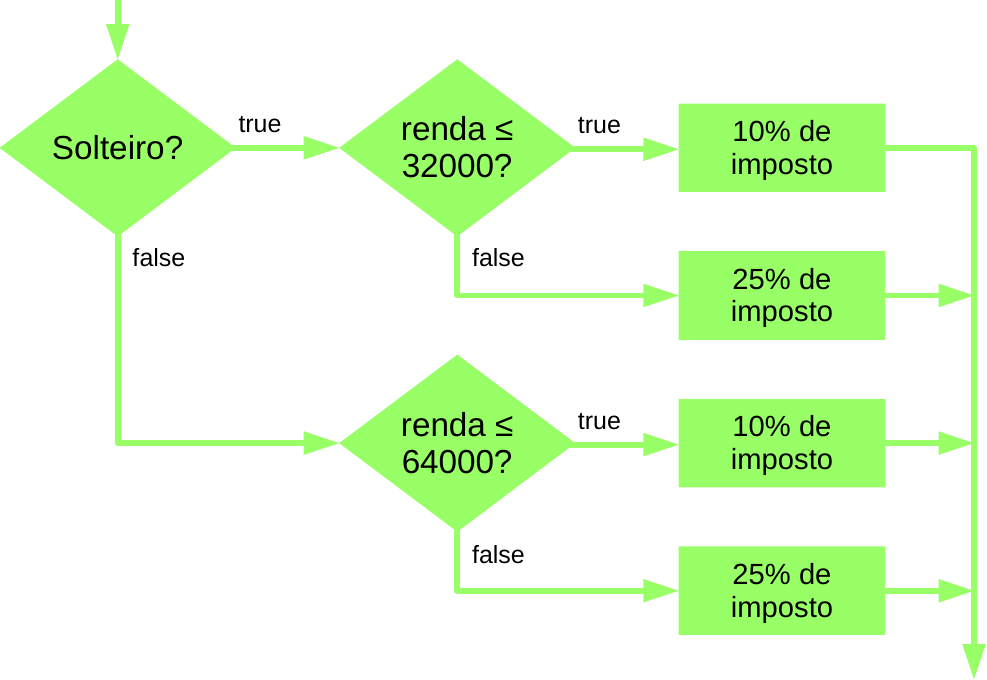
\includegraphics[height=0.65\paperheight,center]{pucrs-ep-fprog-unidade_03-decisoes-laminas-fluxograma_imposto_eua.png}
\end{figure}
\end{center}
\end{frame}

%-------------------------------------------------------
\begin{frame}[fragile]\frametitle{Imposto de Renda nos EUA: implementação}
\tiny{\inputminted[bgcolor=cyan!10]{java}{src/ImpostoEUA.java}}		
\end{frame}

%=======================================================
\section{Exercícios}

%-------------------------------------------------------
\begin{frame}\frametitle{Exercícios (1)}
\begin{enumerate}
	\item Escreva um programa em Java que verifique se um número real é positivo, negativo ou zero.
	\item Tendo como dados de entrada a altura e o sexo de uma pessoa, construa um programa em Java que calcule o seu peso ideal, utilizando as seguintes fórmulas:
	\begin{itemize}
		\item Para mulheres: (62.1 * altura) - 44.7
		\item Para homens: (72.7 * altura) - 58
	\end{itemize}
	\item Escreva um programa em Java que leia o ano de nascimento de uma pessoa, calcule e mostre sua idade, e também verifique e mostre:
	\begin{itemize}
		\item se ela já deve votar (obrigatório para pessoas com idade entre 18 e 70 anos), pode votar (opcional para pessoas com idade entre 16 e 18 anos ou maior que 70 anos) ou não pode votar (impedido para pessoas com idade menor que 16 anos); e
		\item se ela tem idade para conseguir Carteira de Habilitação (18 anos ou mais).
	\end{itemize}
\end{enumerate}
\end{frame}

%-------------------------------------------------------
\begin{frame}\frametitle{Exercícios (2)}
\begin{enumerate}
	\setcounter{enumi}{3}
	\item Escreva um programa em Java que leia o código (inteiro) de um determinado produto e mostre a sua classificação. Utilize as seguintes categorias para classificar os produtos: 1 para ``Alimento não perecível''; 2, 3 ou 4 para ``Alimento perecível''; 5 ou 6 para ``Vestuário''; 7 para ``Higiene pessoal''; e qualquer outro código para ``Inválido''.
\end{enumerate}
\end{frame}

%-------------------------------------------------------
\begin{frame}\frametitle{Exercícios (3)}
\begin{enumerate}
	\setcounter{enumi}{4}
	\item Escreva um programa em Java que leia as 4 notas de um aluno de Fundamentos de Programação ($P_1$, $P_2$, $P_3$ e $M_T$), calcule o seu grau $G_1$ e mostre este grau e uma mensagen indicando se o aluno passou por média ($G_1 \ge 7$), ficou em $G_2$ ($G_1 \ge 4$ e $G_1 < 7$) ou reprovou ($G_1 < 4$). Caso o aluno tenha ficado em $G_2$, calcule qual a nota mínima que o aluno deve tirar nesta prova para obter aprovação.
	Considere que:
	\begin{itemize}
		\item $M_T$ já corresponde à média calculada dos trabalhos e exercícios realizados.
		\item A média de $G_1$ é calculada com a seguinte fórmula:
\[ G_1 = \frac{P_1 + 2 \times P_2 + 3 \times P_3 + M_t}{7} \]
		\item Para obter aprovação depois da realização do $G_2$, a média aritmética entre $G_1$ e $G_2$ deve ser maior ou igual a $5$.
	\end{itemize}
\end{enumerate}
\end{frame}

%-------------------------------------------------------
\begin{frame}\frametitle{Exercícios (4)}
\begin{enumerate}
	\setcounter{enumi}{5}
	\item Escreva um trecho de programa em Java para calcular o número de pontos e o valor de multas de trânsito por excesso de velocidade. Inicialmente seu programa deverá ler o limite de velocidade da via e a velocidade do veículo (medida com um radar), ambos em quilômetros por hora e sem casas decimais. Para determinar a velocidade do veículo que será considerada, aplica-se uma tolerância de 7 km/h, se a velocidade medida for menor ou igual a 100 km/h, ou de 7\%, em caso contrário. Se a velocidade considerada for menor ou igual ao limite da via, não há multa. Se a velocidade considerada exceder 50\% do limite da via, a multa será de R\$880,41 (infração gravíssima, 7 pontos). Se a velocidade considerada exceder 20\% do limite da via, a multa será de R\$195,23 (infração grave, 5 pontos). Senão a multa será de R\$130,16 (infração média, 4 pontos).
\end{enumerate}
\end{frame}

%=======================================================
\section{Referências}

%-------------------------------------------------------
\begin{frame}\frametitle{Referências}
\noindent{HORSTMANN, C. \textbf{Java for Everyone – Late Objetct}. 2. ed. Hoboken: Wiley, 2013. xxxiv, 589 p.}
\end{frame}

%=======================================================
\end{document}

